\documentclass[12pt,a4paper,twoside]{report}
% -------------------------------------------------------------------- %
% Pacotes

\usepackage[utf8]{inputenc}
\usepackage[T1]{fontenc}
\usepackage[brazil]{babel}

\usepackage[fixlanguage]{babelbib}

\usepackage[pdftex]{graphicx}      % usamos arquivos pdf/png como figuras
\usepackage{setspace}              % espaçamento flexvel
\usepackage{indentfirst}           % indentação do primeiro parágrafo
\usepackage{makeidx}               % índice remissivo
\usepackage[nottoc]{tocbibind}     % acrescentamos a bibliografia/indice/conteudo no Table of Contents
\usepackage{courier}               % usa o Adobe Courier no lugar de Computer Modern Typewriter
\usepackage{type1cm}               % fontes realmente escaláveis
\usepackage{titletoc}
\usepackage{ucs}
\usepackage[font=small,format=plain,labelfont=bf,up,textfont=it,up]{caption}
\usepackage[usenames,svgnames,dvipsnames]{xcolor}
\usepackage[a4paper,top=2.54cm,bottom=2.0cm,left=2.0cm,right=2.54cm]{geometry} % margens
\usepackage{amsmath} 

\usepackage[pdftex,plainpages=false,pdfpagelabels,pagebackref,colorlinks=true,citecolor=DarkGreen,
linkcolor=NavyBlue,urlcolor=DarkRed,filecolor=green,bookmarksopen=true]{hyperref} % links coloridos
\usepackage[all]{hypcap}                % soluciona o problema com o hyperref e capítulos
\usepackage[square,sort,nonamebreak,comma]{natbib}  % citação bibliográfica alpha
\fontsize{60}{62}\usefont{OT1}{cmr}{m}{n}{\selectfont}
\usepackage{upquote}                    % formata apóstrofes '
\usepackage{textcomp}

% Para formatar corretamente as URLs
\usepackage{url}
% -------------------------------------------------------------------- %
% Cabeçalhos similares ao TAOCP de Donald E. Knuth
\usepackage{fancyhdr}
\pagestyle{fancy}
\fancyhf{}
\renewcommand{\chaptermark}[1]{\markboth{\MakeUppercase{#1}}{}}
\renewcommand{\sectionmark}[1]{\markright{\MakeUppercase{#1}}{}}
\renewcommand{\headrulewidth}{0pt}

% -------------------------------------------------------------------- %
\graphicspath{{./imagens/}}        % caminho das figuras
\frenchspacing                     % arruma o espaço: id est (i.e.) e exempli gratia (e.g.)
\urlstyle{same}                    % URL com o mesmo estilo do texto e no mono-spaced
\makeindex                         % para o índice remissivo
\raggedbottom                      % para no permitir espaços extras no texto
\fontsize{60}{62}\usefont{OT1}{cmr}{m}{n}{\selectfont}
\cleardoublepage
\normalsize

% -------------------------------------------------------------------- %
% Cores para formatação de código
\usepackage{color}
\definecolor{vermelho}{rgb}{0.6,0,0} % para strings
\definecolor{verde}{rgb}{0.25,0.5,0.35} % para comentários
\definecolor{roxo}{rgb}{0.5,0,0.35} % para palavras-chaves
\definecolor{azul}{rgb}{0.25,0.35,0.75} % para strings
\definecolor{cinza-claro}{gray}{0.95}
% -------------------------------------------------------------------- %
% Opções de listagem usados para o código fonte
% Ref: http://en.wikibooks.org/wiki/LaTeX/Packages/Listings



\usepackage{listings}           % para formatar código-fonte (ex. em Java)


\lstset{ %
language=[Objective]Caml,  % seleciona a linguagem do código (aqui em lstlang0.sty
basicstyle=\footnotesize\ttfamily, % o tamanho da fonte usado no código
commentstyle=\color{verde}\bfseries,  % formatação de comentários
stringstyle=\color{azul},    % formatação de strings
upquote=true,
numbers=left,                   % onde colocar os números de linha
numberstyle=\tiny,  % o tamanho da fonte usada para a numeração das linhas
stepnumber=1,                   % o intervalo entre dois números de linhas. Se for 1, numera cada uma.
numbersep=5pt,                  % how far the line-numbers are from the code
showspaces=false,               % show spaces adding particular underscores
showstringspaces=false,         % underline spaces within strings
showtabs=false,                 % show tabs within strings adding particular underscores
keywordstyle=\color{roxo}\bfseries,
keywordstyle=[1]\color{roxo}\bfseries,
keywordstyle=[2]\color{verde}\bfseries,
%        keywordstyle=[3]\textbf,    %
%        keywordstyle=[4]\textbf,   \sqrt{\sqrt{}} %
frame=b,                   % adds a frame around the code
framerule=0.6pt,
tabsize=2,                      % sets default tabsize to 2 spaces
captionpos=t,                   % sets the caption-position to top
breaklines=true,                % sets automatic line breaking
breakatwhitespace=false,        % sets if automatic breaks should only happen at whitespace
escapeinside={\%*}{*)},         % if you want to add a comment within your code
backgroundcolor=\color[rgb]{1.0,1.0,1.0}, % choose the background color.
rulecolor=\color[rgb]{0.8,0.8,0.8},
extendedchars=true,
xleftmargin=10pt,
xrightmargin=10pt,
framexleftmargin=10pt,
framexrightmargin=10pt,
literate={â}{{\^{a}}}1  % para formatar corretamente os acentos do Português ao usar utf8
    {ê}{{\^{e}}}1
    {ô}{{\^{o}}}1  
    {Â}{{\^{A}}}1
    {Ê}{{\^{E}}}1
    {Ô}{{\^{O}}}1
    {á}{{\'{a}}}1
    {é}{{\'{e}}}1
    {í}{{\'{i}}}1
    {ó}{{\'{o}}}1
    {ú}{{\'{u}}}1
    {Á}{{\'{A}}}1
    {É}{{\'{E}}}1
    {Í}{{\'{I}}}1
    {Ó}{{\'{O}}}1
    {Ú}{{\'{U}}}1
    {à}{{\`{a}}}1
    {À}{{\`{A}}}1
    {ã}{{\~{a}}}1
    {õ}{{\~{o}}}1
    {Ã}{{\~{A}}}1
    {Õ}{{\~{O}}}1
    {ç}{{\c{c}}}1
    {Ç}{{\c{C}}}1
    {ü}{{\"u}}1
    {Ü}{{\"U}}1
}

\renewcommand{\lstlistingname}{Listagem}
\renewcommand{\lstlistlistingname}{Lista de Listagens}

% Definição de novos estilos
\lstdefinestyle{Bash}
    {language=bash,frame=single,numbers=none,basicstyle=\footnotesize\ttfamily,
     morekeywords={cp,mkdir,sudo,tar}}

% Definição de novos ambientes
\lstnewenvironment{terminal}
  {\lstset{style=Bash}}
  {}

\lstnewenvironment{ocaml}
  {\lstset{basicstyle=\scriptsize\ttfamily,
           frame=single,
           frameround=tttt,
           framerule=2pt,
           numbers=none,
           rulecolor=\color{Salmon}}}
  {}

\lstnewenvironment{xml}
   {\lstset{language=XML,frame=single,numbers=none}}
   {}

\lstnewenvironment{interprete}
  {\lstset{frame=single,
            frameround=tttt,
            numbers=none,
            basicstyle=\ttfamily,
            framerule=2pt,
            rulecolor=\color{CadetBlue}}}
  {}
% Formata o caption da listagem
% \DeclareCaptionFont{blue}{\color{blue}} 

% \captionsetup[lstlisting]{singlelinecheck=false, labelfont={blue}, textfont={blue}}
\usepackage{caption}
\DeclareCaptionFont{white}{\color{white}}
\DeclareCaptionFormat{listing}{\colorbox[cmyk]{0.43, 0.35, 0.35,0.01}{\parbox{\textwidth}{\hspace{15pt}#1#2#3}}}
\captionsetup[lstlisting]{format=listing,labelfont=white,textfont=white, singlelinecheck=false, margin=0pt, font={bf,footnotesize}}

\newcommand{\ListingsPath}{./codigos}
% Inclui o nome do arquivo como Caption 
\newcommand{\filelisting}[2][]{%
    \lstinputlisting[caption={\texttt{\detokenize{#2}}},#1]{\ListingsPath/#2}%
}

% ---------------------------------------------------------------------------- %

% ---------------------------------------------------------------------------- %

\title{Construção de um compilador de portugol para Dalvik usando Objective Caml}
\date{}
\author{Guilherme F. O. Martini \\
\texttt{\small \url{guiufo@gmail.com}}\\
\vspace{1cm} \\
Faculdade de Computação \\
Universidade Federal de Uberlândia
}
\date{\today}

%\includeonly{cap-clojure,magical,short}
\begin{document}
  \maketitle
% -------------------------------------------------------------------- %
% Listas de figuras, tabelas e códigos criadas automaticamente
\listoffigures            
\listoftables            
\lstlistoflistings
% -------------------------------------------------------------------- %

% -------------------------------------------------------------------- %
% Sumário
\tableofcontents    

% Capítulos do trabalho

% cabeçalho para as páginas de todos os capítulos
\fancyhead[RE,LO]{\thesection}

%\singlespacing              % espaçamento simples
\setlength{\parskip}{0.15in} % espaçamento entre paragráfos

\chapter{Introdução}
Este trabalho possui o objetivo de documentar a construção de um compilador
de portugol para Dalvik, uma máquina virtual para Android baseada na JVM.
Dalvik foi descontinuado e é parte integral das versões Android até 4.4 (KitKat),
que também contém uma versão beta do ART (Android Runtime).
A partir do Android 5, Dalvik foi completamente substituído pelo ART.

\begin{figure}[h]
	\centering
	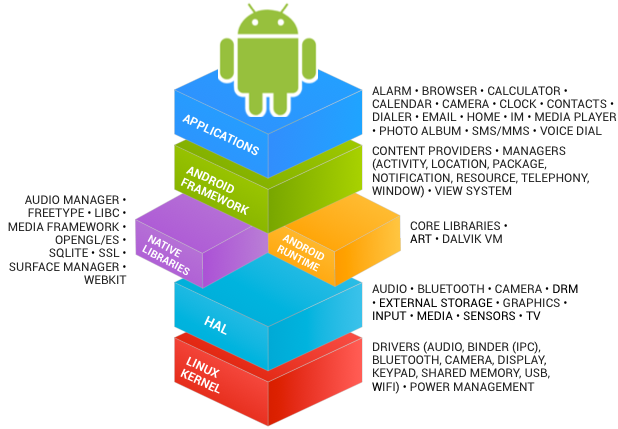
\includegraphics[width=10cm]{imagens/arquitetura-android}
	\caption{Arquitetura Android}
	\label{fig:arquitetura-android}
\end{figure}

\section{Ambiente, Assembler e Disassembler}

Este trabalho foi realizado utilizando GNU/Linux Mint 18 64 Bits.
Esse sistema é baseado em Ubuntu, portanto todos os repositórios e comandos
de instalação são equivalentes nos dois sistemas.

Dalvik utiliza a linguagem smali como assembler. Uma linguagem baseada
em Jasmin, que é um assembler para a JVM. smali gera arquivos .dex, que
podem ser executados na VM de um dispositivo Android, emulado ou real.

Outra ferramenta útil é o Backsmali, que transforma arquivos .dex em
arquivos .smali. smali e Backsmali se encontram na versão 2.2.1 em Agosto de 2017,
e podem ser baixados em formato .jar em \url{https://bitbucket.org/JesusFreke/smali/downloads/.}.

Considere um programa "Hello World!" para smali:

% Programa "Hello World!" para smali
\lstinputlisting[label={arq:HelloWorld.smali}, language=Java,
caption={HelloWorld.smali}]{codigos/smali/HelloWorld.smali}

Para gerarmos um arquivo .dex:
\begin{terminal}
> java -jar smali.jar assemble HelloWorld.smali -o HelloWorld.dex
\end{terminal}

Para decompilar o arquivo .dex gerado para a pasta "out":
\begin{terminal}
> java -jar baksmali.jar disassemble HelloWorld.dex
\end{terminal}

Para executar um arquivo .dex é necessário entrar no AndroidStudio,
criar um dispositivo virtual com Android 4.4 ou menor e então iniciar o dispositivo.
Daí podemos executar os seguintes comandos (adb espera um arquivo classes.dex):
\begin{terminal}
> zip HelloWorld.zip classes.dex
> adb push HelloWorld.zip /data/local
> adb shell dalvikvm -cp /data/local/HelloWorld.zip HelloWorld
Hello World!
\end{terminal}

\section{Arquitetura Dalvik e Dalvik Bytecode}

\subsection{Dalvik}
O Dalvik é uma máquina virtual java modificada para rodar o Android. Uma das diferenças do
Dalvik para ART é que ART usa um arquivo DEX modificado, que contém código nativo (Fig. \ref{fig:arquitetura-dalvik}).

\begin{figure}[h]
	\centering
	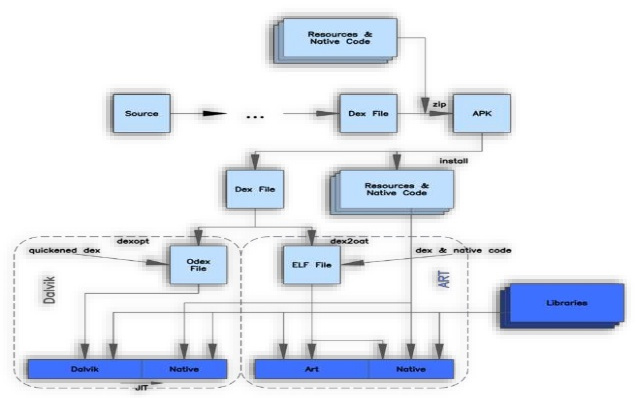
\includegraphics[width=10cm]{imagens/arquitetura-dalvik}
	\caption{Arquitetura Dalvik}
	\label{fig:arquitetura-dalvik}
\end{figure}

\subsection{Bytecode}
A máquina virtual Dalvik é parecida com as arquiteturas reais mais comuns. As chamadas de função são ao estilo da linguagem C.  A máquina é baseada em registros e frames de tamanho fixo, e contém as seguintes
características.

\begin{enumerate}
	\item Um frame contém os registros de um método e os metadados para a execução, como o contador de programa e a referência para o .dex que contém o método.
	\item Um registro contém 32 bits. Um dado de 64 bits usa dois registradores de 32 bits.
	\item Os N argumentos de um método ficam nos últimos N registros do frame do método de invocação, em ordem.
\end{enumerate}

\chapter{Compilador}

\section{Arquitetura}
Estamos construindo um compilador de portugol para Dalvik. Estamos seguindo uma arquitetura
tradicional (Fig \ref{fig:arquitetura-compilador}). Não estamos fazendo qualquer otimização, e foi
implementado um intérprete, que usa uma árvore sintática tipada para avaliar o código.
Uma maneira mais adequada de implementar o intérprete seria através da análise do código de 3 endereços. Assim teríamos
um interpretador geral, independente da linguagem fonte.

\begin{figure}[h]
	\centering
	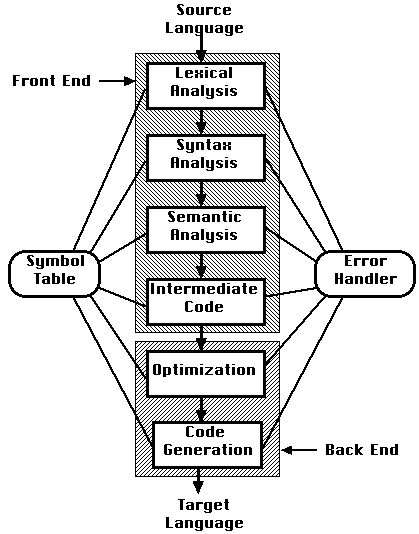
\includegraphics[width=10cm]{imagens/arquitetura-compilador}
	\caption{Arquitetura geral de um compilador}
	\label{fig:arquitetura-compilador}
\end{figure}

\section{Analisador Léxico}

\subsection{Apresentação}
O analisador léxico é o único elemento do compilador que analisa todo o código, caractere por caractere.
Ele é reponsável por eliminar os espaços em branco e comentários. O analisador lê o código e retorna uma
lista de tokens, formados pelos lexemas possíveis da linguagem fonte.

\subsection{Implementação}

O analisador é escrito no arquivo lexer.mll, que é compilado para lexing.ml e utilizado para gerar a lista de tokens.
Segue o código da implementação do analisador:

\lstinputlisting[label={arq:lexer.mll}, language=Caml,
caption={lexer.mll}]{codigos/ocaml/lexer.mll}

\subsection{Utilização}

O arquivo lexer.mll é compilador usando o programa Ocamllex, cujos códigos .mll possuem uma sintaxe
própria, otimizada para a descrição de analisadores léxicos. Para a compilação do projeto estamos usando o ocamlbuild, um projeto
parecido com o make, que facilita o processo de compilação. Além disso, para carregar arquivos quando o ocaml inicia, usamos
o arquivo .ocamlinit, que sempre executa quando iniciamos o ocaml. Para compilar o analisador:

\begin{terminal}
> ocamllex lexer.mll
> ocamlc lexer.ml
\end{terminal}

\section{Analisador Sintático}

O analisador sintático foi implementado usando o Menhir, um construtor de analisadores sintáticos do tipo LR(1). Nessa fase definimos
uma gramática e um componente para a construção de uma árvore sintática abstrata, utilizada para a construção dos elementos que irão compor a árvore, como operadores, literais e funções. O analisador recebe uma lista de tokens e retorna uma árvore sintática abstrata, construída à partir da gramática
(Fig \ref{fig:parsing}).

\begin{figure}[h]
	\centering
	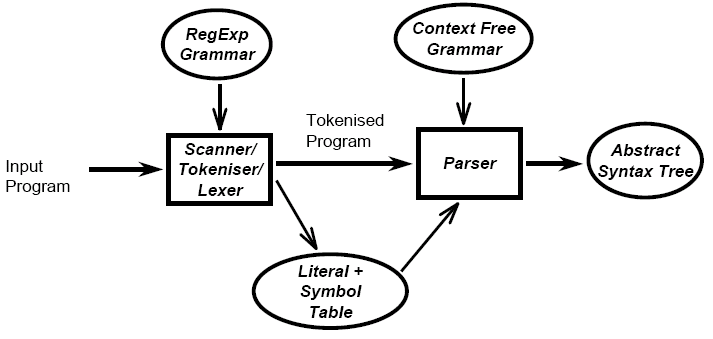
\includegraphics[width=10cm]{imagens/parsing}
	\caption{Analisador Sintático}
	\label{fig:parsing}
\end{figure}

\subsection{Implementação}

O modelo da árvore sintática está definido no arquivo ast.ml. O parser em si é definido no arquivo parser.mly. É gerado um autômato
juntamente com um arquivo de mensagens de erros, que deve ser modificado para retornar as mensagens desejadas para os erros. Além
disso temos o arquivo sintaticoTest.ml, capaz de receber um arquivo, passando pelo scanner e pelo parser e gerando o autômato.
Segue os códigos dos arquivos apresentados.

\begin{enumerate}

\item{parser.mly}
\lstinputlisting[label={arq:parser.mly}, language=Caml,
caption={parser.mly}]{codigos/ocaml/parser.mly}

\item{sintaticoTest.ml}
\lstinputlisting[label={arq:parser.ml}, language=Caml,
caption={sintaticoTest.ml}]{codigos/ocaml/sintaticoTest.ml}
\end{enumerate}

\subsection{Utilização}

Para compilar o parser usamos os seguintes comandos:
\begin{terminal}
> menhir -v --list-errors sintatico.mly > sintatico.msg
> menhir -v --list-errors sintatico.mly --compile-errors sintatico.msg > erroSint.ml
> ocamlbuild -use-menhir sintaticoTest.byte
\end{terminal}

Então podemos usar a função parse\_arq para ler um arquivo e gerar a árvore:

\begin{figure}[h]
	\centering
	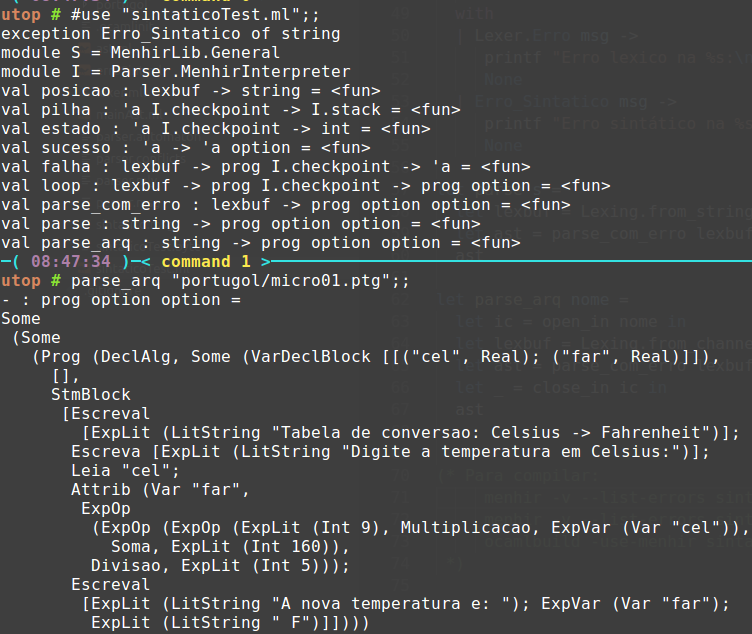
\includegraphics[width=10cm]{imagens/sintatico-test}
	\caption{Usando o Analisador Sintático}
	\label{fig:parsing}
\end{figure}

\section{Analisador Semântico}
O analisador semântico é responsável por gerar uma árvore sintática abstrata tipada, verificando se não há conflitos
em operações, expressões e comandos. 

\subsection{Implementação}

\subsection{Utilização}


\section{Intérprete}

\subsection{Implementação}

\subsection{Utilização}


\section{Representação Intermediária}

\subsection{Implementação}

\subsection{Utilização}


\section{Tradução para bytecode}

\subsection{Implementação}

\subsection{Utilização}


\chapter{Códigos}

\section{portugol e smali}
Listagem de programas portugol e respectivas traduções para smali:
\begin{enumerate}
% Nano01
\item nano01.ptg
\lstinputlisting[label={arq:nano01.ptg}, language=Java,
caption={nano01.ptg}]{codigos/portugol/nano01.ptg}

\item Nano01.smali
\lstinputlisting[label={arq:Nano01.smali}, language=Java,
caption={Nano01.smali}]{codigos/smali/Nano01.smali}

% Nano02
\item nano02.ptg
\lstinputlisting[label={arq:nano02.ptg}, language=Java,
caption={nano02.ptg}]{codigos/portugol/nano02.ptg}

\item Nano02.smali
\lstinputlisting[label={arq:Nano02.smali}, language=Java,
caption={Nano02.smali}]{codigos/smali/Nano01.smali}

% Nano03
\item nano03.ptg
\lstinputlisting[label={arq:nano03.ptg}, language=Java,
caption={nano03.ptg}]{codigos/portugol/nano03.ptg}

\item Nano03.smali
\lstinputlisting[label={arq:Nano03.smali}, language=Java,
caption={Nano03.smali}]{codigos/smali/Nano03.smali}

% Nano04
\item nano04.ptg
\lstinputlisting[label={arq:nano04.ptg}, language=Java,
caption={nano04.ptg}]{codigos/portugol/nano04.ptg}

\item Nano04.smali
\lstinputlisting[label={arq:Nano04.smali}, language=Java,
caption={Nano04.smali}]{codigos/smali/Nano04.smali}

% Nano05
\item nano05.ptg
\lstinputlisting[label={arq:nano05.ptg}, language=Java,
caption={nano05.ptg}]{codigos/portugol/nano05.ptg}

\item Nano05.smali
\lstinputlisting[label={arq:Nano05.smali}, language=Java,
caption={Nano05.smali}]{codigos/smali/Nano05.smali}

% Nano06
\item nano06.ptg
\lstinputlisting[label={arq:nano06.ptg}, language=Java,
caption={nano06.ptg}]{codigos/portugol/nano06.ptg}

\item Nano06.smali
\lstinputlisting[label={arq:Nano06.smali}, language=Java,
caption={Nano06.smali}]{codigos/smali/Nano06.smali}

% Nano07
\item nano07.ptg
\lstinputlisting[label={arq:nano07.ptg}, language=Java,
caption={nano07.ptg}]{codigos/portugol/nano07.ptg}

\item Nano07.smali
\lstinputlisting[label={arq:Nano07.smali}, language=Java,
caption={Nano07.smali}]{codigos/smali/Nano07.smali}

% Nano08
\item nano08.ptg
\lstinputlisting[label={arq:nano08.ptg}, language=Java,
caption={nano08.ptg}]{codigos/portugol/nano08.ptg}

\item Nano08.smali
\lstinputlisting[label={arq:Nano08.smali}, language=Java,
caption={Nano08.smali}]{codigos/smali/Nano08.smali}

% Nano10
\item nano10.ptg
\lstinputlisting[label={arq:nano10.ptg}, language=Java,
caption={nano10.ptg}]{codigos/portugol/nano10.ptg}

\item Nano10.smali
\lstinputlisting[label={arq:Nano10.smali}, language=Java,
caption={Nano10.smali}]{codigos/smali/Nano10.smali}

% Nano11
\item nano11.ptg
\lstinputlisting[label={arq:nano11.ptg}, language=Java,
caption={nano11.ptg}]{codigos/portugol/nano12.ptg}

\item Nano11.smali
\lstinputlisting[label={arq:Nano11.smali}, language=Java,
caption={Nano11.smali}]{codigos/smali/Nano11.smali}

% Nano12
\item nano12.ptg
\lstinputlisting[label={arq:nano12.ptg}, language=Java,
caption={nano12.ptg}]{codigos/portugol/nano12.ptg}

\item Nano12.smali
\lstinputlisting[label={arq:Nano12.smali}, language=Java,
caption={Nano12.smali}]{codigos/smali/Nano12.smali}

% Micro01
\item micro01.ptg
\lstinputlisting[label={arq:micro01.ptg}, language=Java,
caption={micro01.ptg}]{codigos/portugol/micro01.ptg}

\item Micro01.smali
\lstinputlisting[label={arq:Micro01.smali}, language=Java,
caption={Micro01.smali}]{codigos/smali/Micro01.smali}

% Micro02
\item micro02.ptg
\lstinputlisting[label={arq:micro02.ptg}, language=Java,
caption={micro02.ptg}]{codigos/portugol/micro02.ptg}

\item Micro02.smali
\lstinputlisting[label={arq:Micro02.smali}, language=Java,
caption={Micro02.smali}]{codigos/smali/Micro02.smali}

% Micro03
\item micro03.ptg
\lstinputlisting[label={arq:micro03.ptg}, language=Java,
caption={micro03.ptg}]{codigos/portugol/micro03.ptg}

\item Micro03.smali
\lstinputlisting[label={arq:Micro03.smali}, language=Java,
caption={Micro03.smali}]{codigos/smali/Micro03.smali}


% Micro04
\item micro04.ptg
\lstinputlisting[label={arq:micro04.ptg}, language=Java,
caption={micro04.ptg}]{codigos/portugol/micro04.ptg}

\item Micro04.smali
\lstinputlisting[label={arq:Micro04.smali}, language=Java,
caption={Micro04.smali}]{codigos/smali/Micro04.smali}


% Micro05
\item micro05.ptg
\lstinputlisting[label={arq:micro05.ptg}, language=Java,
caption={micro05.ptg}]{codigos/portugol/micro05.ptg}

\item Micro05.smali
\lstinputlisting[label={arq:Micro05.smali}, language=Java,
caption={Micro05.smali}]{codigos/smali/Micro05.smali}

% Micro06
\item micro06.ptg
\lstinputlisting[label={arq:micro06.ptg}, language=Java,
caption={micro06.ptg}]{codigos/portugol/micro06.ptg}

\item Micro06.smali
\lstinputlisting[label={arq:Micro06.smali}, language=Java,
caption={Micro06.smali}]{codigos/smali/Micro06.smali}

% Micro07
\item micro07.ptg
\lstinputlisting[label={arq:micro07.ptg}, language=Java,
caption={micro07.ptg}]{codigos/portugol/micro07.ptg}

\item Micro07.smali
\lstinputlisting[label={arq:Micro07.smali}, language=Java,
caption={Micro07.smali}]{codigos/smali/Micro07.smali}

% Micro08
\item micro08.ptg
\lstinputlisting[label={arq:micro08.ptg}, language=Java,
caption={micro08.ptg}]{codigos/portugol/micro08.ptg}

\item Micro08.smali
\lstinputlisting[label={arq:Micro08.smali}, language=Java,
caption={Micro08.smali}]{codigos/smali/Micro08.smali}

% Micro09
\item micro09.ptg
\lstinputlisting[label={arq:micro09.ptg}, language=Java,
caption={micro09.ptg}]{codigos/portugol/micro09.ptg}

\item Micro09.smali
\lstinputlisting[label={arq:Micro09.smali}, language=Java,
caption={Micro09.smali}]{codigos/smali/Micro09.smali}

% Micro10
\item micro10.ptg
\lstinputlisting[label={arq:micro10.ptg}, language=Java,
caption={micro10.ptg}]{codigos/portugol/micro10.ptg}

\item Micro10.smali
\lstinputlisting[label={arq:Micro10.smali}, language=Java,
caption={Micro10.smali}]{codigos/smali/Micro10.smali}

% Micro11
\item micro11.ptg
\lstinputlisting[label={arq:micro11.ptg},
caption={micro11.ptg}]{codigos/portugol/micro11.ptg}

\item Micro11.smali
\lstinputlisting[label={arq:Micro11.smali}, language=Java,
caption={Micro11.smali}]{codigos/smali/Micro11.smali}

\end{enumerate}

\chapter{Referências}


\clearpage
\addcontentsline{toc}{part}{Apêndice}
\appendix

\end{document} 
